\section{Introduction}
The WLCG strategy paper \cite{wlcgstrategy} set out the path towards computing for the High-Luminosity LHC (HL-LHC) era, building up from the input provided by the HSF \cite{hsf} Community White Paper \cite{cwp}.
The estimates for the data volumes and computing show a major step up from the current needs and a program of work was established from the WLCG point of view to address this future challenge. One of the charges is addressed by the DOMA Access Working Group to evaluate future data access scenarios.\\
During the first year, the DOMA Access Working Group collected information from the experiments about the evolution of their computing models and future plans for user data analysis.\\
The working group is investigating the potential benefits of data caching infrastructures and promoting their deployment within a consolidated storage infrastructure labeled as WLCG-Data Lake (Fig. ~\ref{datalake-concept}), from now on referred to as Data Lake.
%\footnote{Following-up the work pioneered by the cost model working group \cite{costmodel} to understand file placement and file usage statistics} 

\begin{figure}
  \centering
  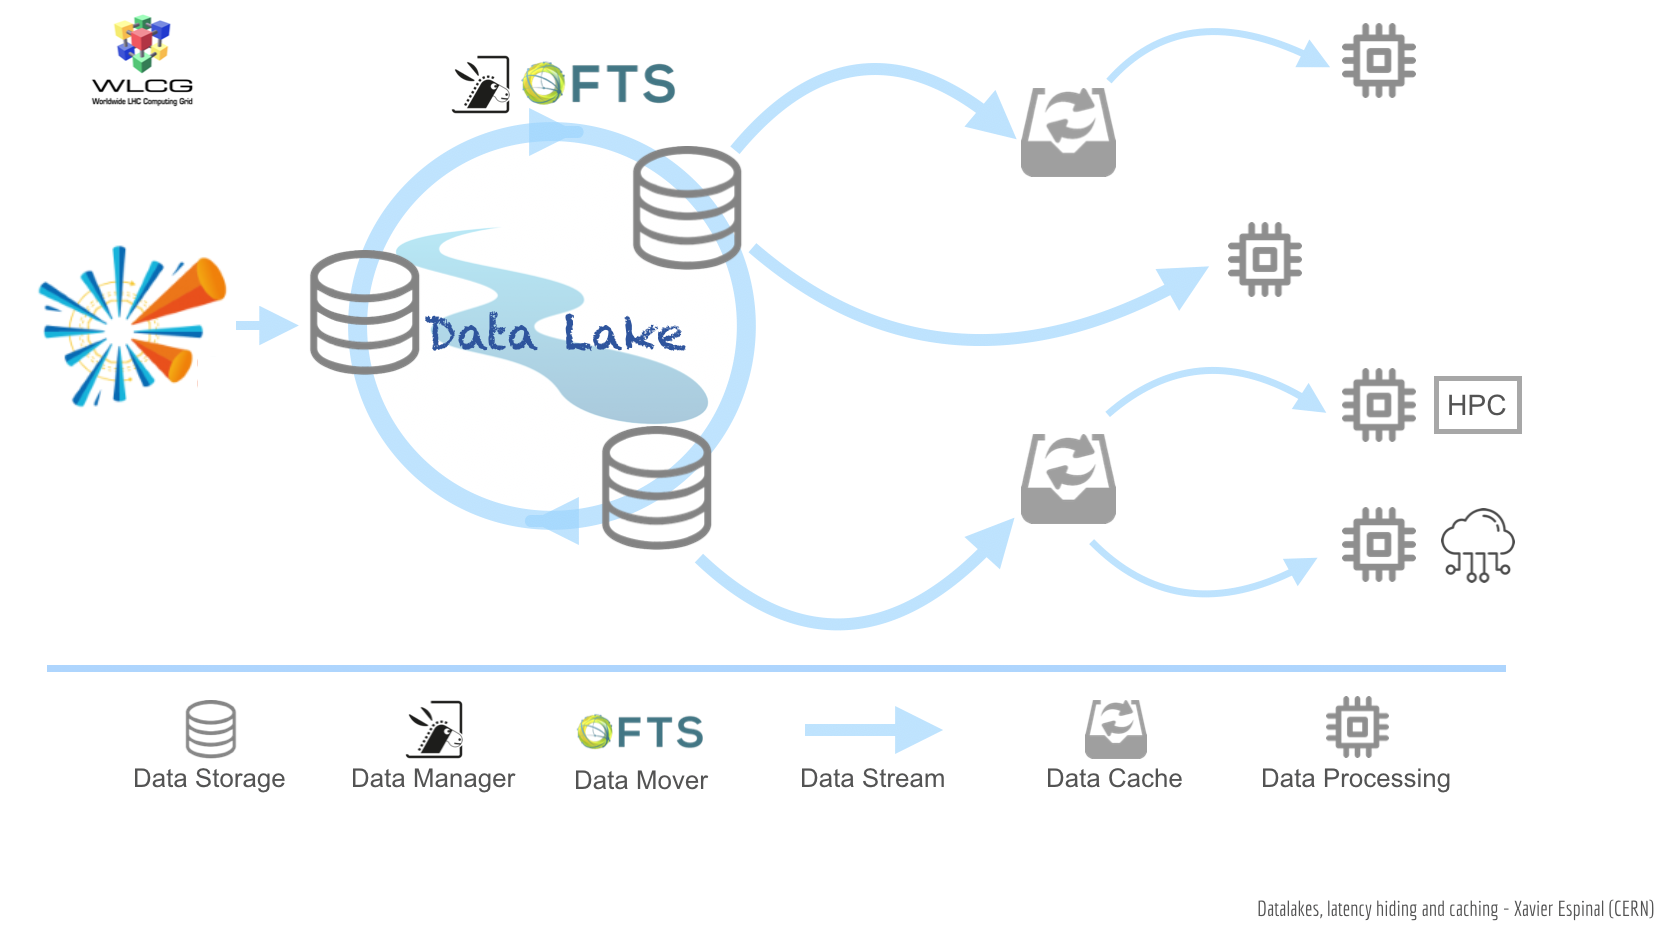
\includegraphics[height=6cm]{datalake-concept-sketch.png}
  \caption{{\em} Conceptual sketch of the WLCG-Data Lake }
  \label{datalake-concept}
\end{figure}



